\chapter{Background}\label{chap:background}

This case study was performed at 30MHz, specifically within the context of their software platform. This section describes the company (30MHz), their software platform (the dashboard), and the problem solved by the case study.

\section{The Company}\label{sec:bg:thecompany}
30MHz is a technology company in the agriculture industry. They offer sensors that collect various types of data, all within the context of agriculture. Examples of types of data include temperature, humidity, and air pressure. 30MHz also provides their customers with a dashboard that allows them to view the collected data. An example of this dashboard can be seen in Figure~\ref{fig:bg:dashboard}. This dashboard is a web app that, as of this case study, is using Angular 10. Data is fetched from a backend, and the various types of data are displayed in different ways using so-called widgets. There are currently three types of widgets:

\begin{itemize}
  \item \emph{Chart:} A chart widget displays the value of the data over time and provides a good overview of the history of the data up to a given point. An example of a chart can be seen in Figure~\ref{fig:bg:dashboard} in all but the top-right section.
  \item \emph{Gauge:} Gauge widgets display the current value of a sensor in a given range. It allows the user to see whether the current value is still within the correct range. An example of a gauge widget can be found on the top-right in Figure~\ref{fig:bg:dashboard}.
  \item \emph{Image:} Image widgets display the value of a sensor on a specific location of an image. This widget can be used to, for example, display the temperature at various sites on a map. An example of an image widget can be found in Figure~\ref{fig:bg:dashboard-img}.
\end{itemize}

\begin{figure}[h]
  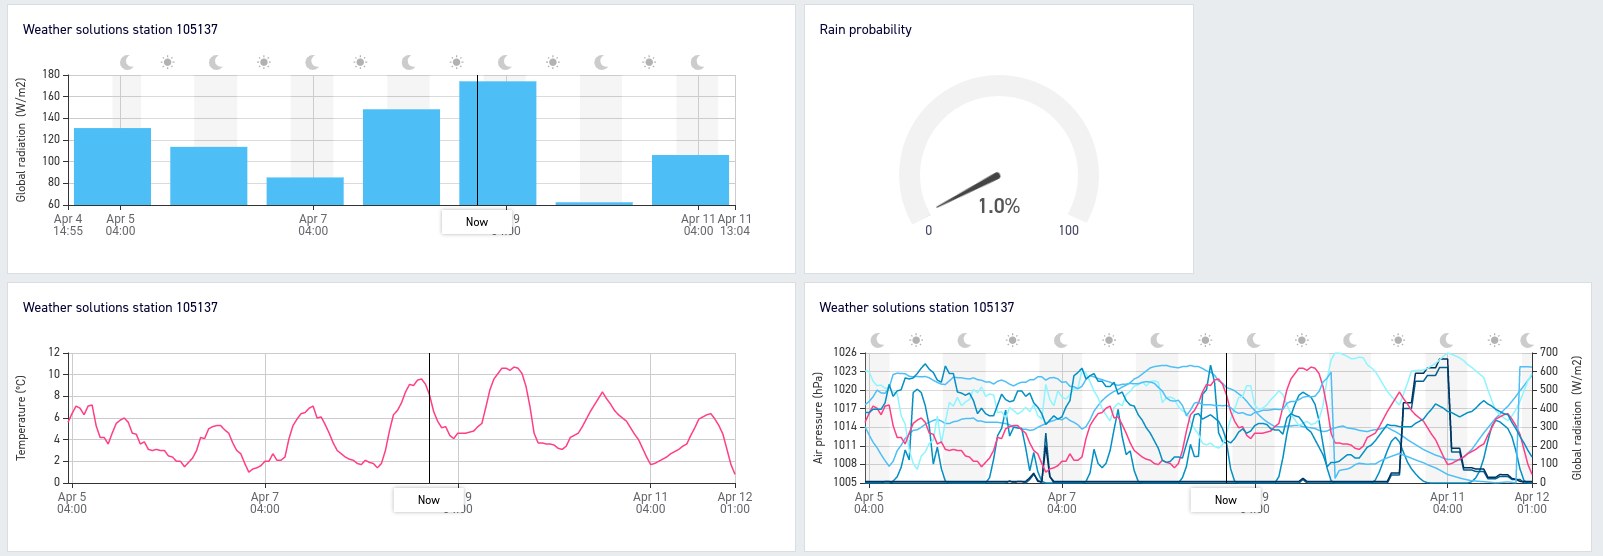
\includegraphics[width=\columnwidth]{figures/background/dashboard.png}
  \caption{Widgets in the 30MHz dashboard}
  \label{fig:bg:dashboard}
  \centering
\end{figure}

\begin{figure}[h]
  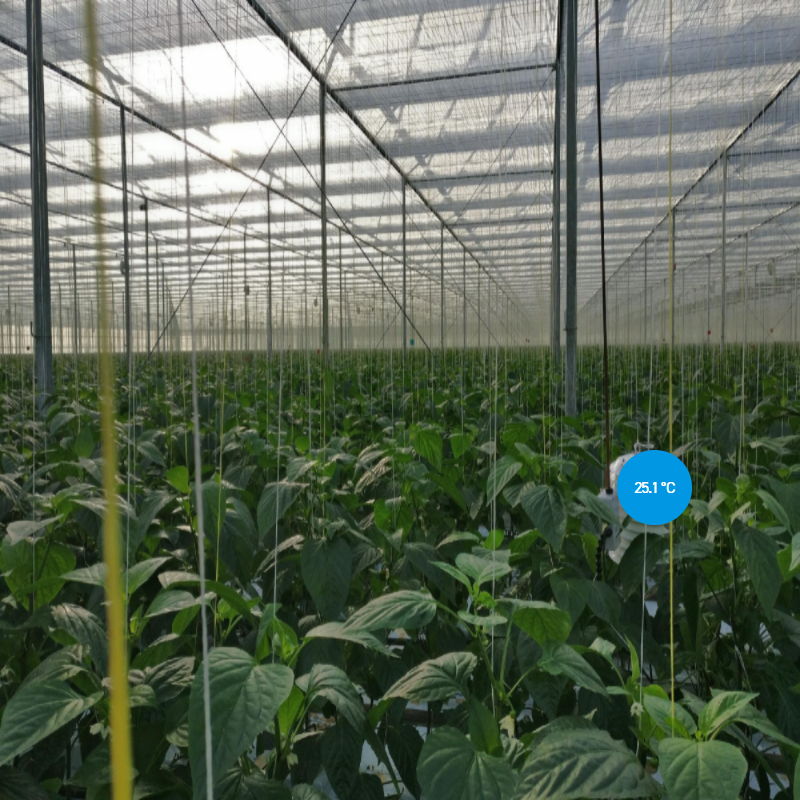
\includegraphics[width=\columnwidth]{figures/background/dashboard-img.png}
  \caption{An image widget in the 30MHz dashboard}
  \label{fig:bg:dashboard-img}
  \centering
\end{figure}

\subsection{Apps}\label{sec:bg:apps}
The data collected by 30MHz can be utilized in many ways. Companies with domain knowledge and expertise in certain areas (such as third parties) can provide customers with new insights and information that simple graphs can not. Because 30MHz itself does not have this domain knowledge and does not have the resources to create every single possible implementation of this knowledge (in the form of a widget or page in the dashboard), 30MHz decided to allow third-party developers to develop them instead. There are currently two implementations:

\begin{itemize}
  \item \emph{Widgets:} A Widget in the dashboard takes data from one or more sensors and displays it. These are made to provide information at a glance and are fairly small when it comes to screen space, as can be seen in Figure~\ref{fig:bg:dashboard}. An example would be a new way to display the amount of light a plant is getting by showing a sun icon if the plants can grow (it is daytime) and a moon icon if they can not (it is nighttime).
  \item \emph{Apps:} Apps are full pages in the web app. These fill the entire screen (bar some 30MHz branding) and provide richer and more interactive experiences. An example would be a page where users can tune parameters (such as the number of crops, amount of watering) and see a prediction of their revenue. This prediction can be based (in part) on sensor data.
\end{itemize}

Since these apps will essentially be pages in the 30MHz dashboard and will feel like part of the platform, it is important that they follow the same design as the rest of the dashboard. A consistent design ensures that users are familiar with the apps and that visual consistency across the platform is not broken. This concept has been applied on Google's Android through Material Design~\footurl{https://material.io/} and Zendesk Garden~\footurl{https://garden.zendesk.com/} among others. Importantly, these companies all provide app developers with a set of components to help them maintain the intended design language. Such a set of components is generally referred to as a UI library.
Similarly, 30MHz wants to provide their third-party app developers with a UI library. In this paper, we will refer to the UI library 30MHz will provide to third parties as the Cow Components UI Library (or CC UI Library). It is named after the logo of 30MHZ, a cow. There already is an internal UI library that covers the basic set of UI components (among others buttons, an input, a date picker), but since it is interwoven with other internal code, its source code can not just be provided to third-party developers. Additionally, they have been written in Angular~\footurl{https://angular.io/}, meaning that any developers who wish to develop their app in a different JavaScript (JS) framework cannot do so. Looking at the most popular web frameworks in the latest Stack Overflow Developer Survey~\footurl{https://insights.stackoverflow.com/survey/2020} (2020 as of the writing of this paper), we can conclude that the chance that a developer wishes to use a different JS framework is quite large. In order to still provide developers with a CC UI library, there are two options.

\begin{itemize}
  \item Write components from scratch in a framework-agnostic format and provide them to developers. Then keep them up to date with the internal set of components by changing one as the other changes.
  \item Set up automatic migration from the set of internal components to a framework-agnostic format.
\end{itemize}

The immediately apparent problem with the first option is that developers are maintaining two separate copies of very similar code. This causes several issues. Firstly, the time spent maintaining a component is doubled. Additionally, feature differences between the Angular framework and the framework-agnostic format we choose will lead to added engineering time. Some things that make use of the Angular framework might need workarounds in the other format and the other way around. Another issue with the first option is that the components have to be written entirely from scratch. While writing components from scratch would be manageable for simple components such as buttons, it is unfeasible for more complex components. One such component for which the rewriting process would prove difficult is the 30MHz chart component. This component is vital to the 30MHz design library, seeing as it displays the sensor data. The source code for the chart is tightly coupled with the rest of the platform, referencing about half of the source files in the dashboard through its dependencies. Rewriting all of this code in another framework is wholly unfeasible and not worth the effort, leading us to explore the second option.

While the second option is not an easy one and will likely be a very complex process to set up, it will scale a lot better. Once it is set up, any new components will be automatically migrated, and any changes will be propagated automatically. In the long run, this automatic migration should save time. This option is the one 30MHz eventually decided on. Next, a framework-agnostic format needs to be chosen to facilitate this process.

\section{Web Components}\label{sec:bg:webcomponents}
When it comes to choosing a framework-agnostic format for a UI library, there are very few options. Looking at the literature, we find Quid~\cite{molina2019quid}, a program that allows code written in a domain-specific language (DSL) to be used to generate components in various frameworks. It currently supports the generating of Web Components~\footurl{https://developer.mozilla.org/en-US/docs/Web/Web_Components}, Stencil~\footurl{https://stenciljs.com/}, Angular and Polymer~\footurl{https://www.polymer-project.org/} components. The authors do mention it should only be used for rapid prototyping. Since it only supports a fairly small set of supported frameworks, and it has the problem of requiring a DSL which the Angular code would have to be migrated to, we choose not to use Quid as the target format.

This brings us to another option, namely Web Components. Web Components (also known as Custom Elements) are a technology proposed in 2013~\footurl{https://www.w3.org/TR/2013/WD-custom-elements-20130514/\#about} and implemented in major browsers in 2018~\footurl{https://caniuse.com/?search=webcomponents}. It allows for the creation of custom HTML elements using JavaScript. These elements can then be used like regular HTML elements. Since every JS framework has support for native HTML elements and almost every framework has full support for Web Components~\footurl{https://custom-elements-everywhere.com/}, we can cover most JS frameworks by using Web Components as our target format.

\section{Angular Elements}\label{sec:bg:angularelements}
To perform the migration of Angular components to Web Components, we use Angular Elements~\footurl{https://angular.io/guide/elements}. Angular Elements is a JS package that allows for the migration of Angular components to Web Components. It does this by changing the way in which components are mounted. Angular apps are typically mounted to the page by the user through a call to the \code{bootstrapModule} function. Consequently, the bootstrap component is mounted to the page. This bootstrap component is responsible for containing the rest of the application. After it is mounted, child components are mounted and rendered within its root recursively. Angular Elements works slightly differently. Components registered as Web Components through Angular Elements are instead rendered whenever an HTML element with the registered tag is added to the DOM\@ (document object model). The DOM is the model containing the elements on a page and how they are positioned relative to each other. Adding an element to the DOM adds it to the webpage. When such a component is rendered, a new root is created in place of this new HTML element. Instead of a single root in which everything is rendered (as is the case in a typical Angular app), components are all rendered in their own local root. We use Angular Elements for the migration to Web Components in this case study since it appears to be the only package providing this capability.

\begin{figure}[h]
  \caption{An example of a component that provides type hints (these hints are also referred to as intellisense)}
  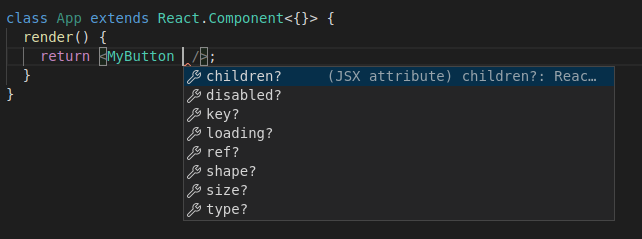
\includegraphics[width=\columnwidth]{figures/background/hinting.png}
  \label{fig:bg:hinting}
  \centering
\end{figure}

\begin{figure}[h]
  \caption{An example of a component without type hints}
  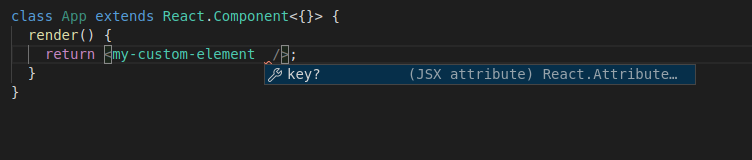
\includegraphics[width=\columnwidth]{figures/background/no-hinting.png}
  \label{fig:bg:no-hinting}
  \centering
\end{figure}

\begin{figure}[h]
  \caption{A diagram representing the relationship between the JS framework and Web Components}
  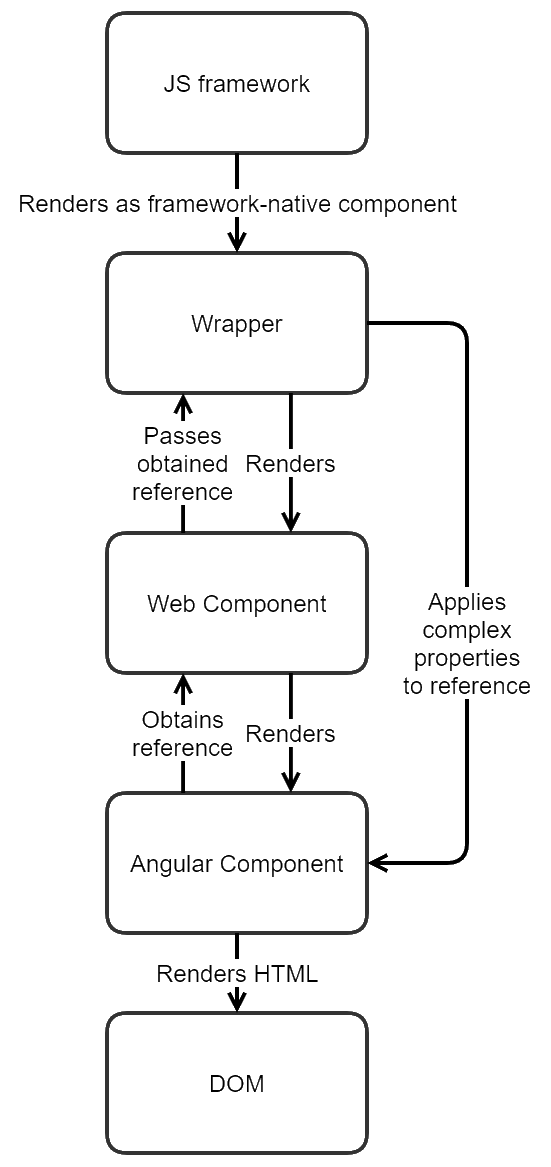
\includegraphics[scale=0.3]{figures/background/wrapper-diagram.png}
  \label{fig:bg:wrapper-diagram}
  \centering
\end{figure}


\section{Javascript frameworks}\label{sec:bg:jsframeworks}
While migrating components to Web Components makes them usable in most JS frameworks, they do not provide a perfect experience. The first reason for this is them not being perfectly compatible with every JS framework. As of the writing of this paper, there are still some issues preventing them from working entirely in ReactJS~\footurl{https://reactjs.org/}, a JS framework created by Facebook in 2013. These issues mostly concern the passing of non-primitive data to the components, such as JavaScript Objects, Arrays, and Functions. The second problem is that they are not native to JS frameworks and do not integrate very well with the tooling provided by the framework. One such tool is type hinting, in which an editor suggests possible values to the developer. An example of type hinting provided by the framework and editor can be seen in Figure~\ref{fig:bg:hinting}. Compared to Figure~\ref{fig:bg:no-hinting}, which shows a component with no type hinting, Figure~\ref{fig:bg:hinting} provides the developer with much more information and shows them what options are available to them. Instead of searching the web for the available properties, these options are provided by the element's source code and displayed through the framework's tooling and the editor. In order to improve the developer experience, we will provide what we will call a \emph{wrapper} for each framework. This wrapper has two functions. Firstly, it provides the tooling mentioned above. Secondly, it bridges the gap with JS frameworks that do not natively support Web Components yet. This wrapper is native to the framework, being written using the language and library the framework provides. This allows the framework to infer information from the wrapper's source code. Under the hood, this wrapper still uses the components in the Web Components UI library to render the components. This wrapper serves as glue code between the framework and these components. By combining the two steps of migrating the original Angular components to Web Components, and the Web Components to wrappers for frameworks, we can provide developers with an experience native to their framework, even though the original source code uses Angular. An overview layout of the relationship between the JS framework, the wrapper and the Web Components can be seen in Figure~\ref{fig:bg:wrapper-diagram}.

\section{UI Libraries}\label{sec:bg:ui-libraries}
As mentioned before, a set of components that adheres to one cohesive design language is generally referred to as a UI library or design library. There are two methods for implementing a design library, with one being based on doing most of the work in JavaScript and the other being based on shifting this work to CSS. The former is also referred to as a design library, with the latter being called a CSS framework. The idea of a CSS framework is to put almost all of the styles a developer will need in a single CSS file. This includes the various variations they could need. For example, a CSS library could include the \code{.padding-5} selector as well as the \code{.padding-2} selector for setting the padding of a component. Note that the number of pixels of this padding is included in the selector. This generally leads to relatively big CSS files, which may or may not be tree shaken. This is in contrast to JavaScript-based UI libraries, which generally use per-component stylesheets instead of global stylesheets. They also tend to shift numbers and sizes to JavaScript or HTML\@. For example the same padding as above could be applied through a property, i.e. \code{<my-component padding="2"/>} or \code{<my-component padding="5"/>}. This approach has the advantage of a more per-component focus, more flexibility, and options that are easier to discover. However, compared to CSS frameworks, JS-based UI libraries are significantly slower. The CSS frameworks generally only append an element to the DOM and apply some pre-computed set of classes to them, meaning they only interact with the swift JavaScript APIs that are native to the browser. JS-based UI libraries, on the other hand, have to take care of styling, component interactivity through various event listeners, and changing what is rendered depending on properties. Since this performance difference is important when it comes to measurements, a given library being a UI library or CSS framework, is mentioned later.
